% ILP (for ICS'05)
%
%\documentclass[10pt,dvips]{article}
\documentclass[10pt,dvips]{article}
%\documentclass[10pt,twocolumn,dvips]{article}
\usepackage[english]{babel}
\usepackage{epsfig}
%\usepackage{fancyheadings}
%\usepackage[T1]{fontenc}
%\usepackage[latin1]{inputenc}
%\usepackage{twocolumn}
%\usepackage{verbatim,moreverb,doublespace}
%\usepackage{rotate,lscape,dcolumn,array,rotating,latexsym}
%
%\input{epsf}
%
% for (IEEE single-column format)
%\textwidth 6.875in
%\textheight 8.875in
%\topmargin -0.6in
%\oddsidemargin 0mm
%\evensidemargin 0mm
%
% for HPCA (IEEE two-column format)
%\textwidth 6.5in
%\textheight 8.875in
%\topmargin -0.4in
%\oddsidemargin 0mm
%\evensidemargin 0mm
%
% for ICS05
\textwidth 6.5in
\textheight 8.875in
\topmargin -0.4in
\oddsidemargin 0mm
\evensidemargin 0mm
%
%
% turn the following (linespread) on to 1.6 for "double space"
\linespread{1.6}
%
%
% some publishers want no page numbers for final print
%\pagestyle{empty}
%
\begin{document}
%
%
\title{Targeting the ILP Wall}
%
%
\author{
undisclosed
}
%
%
% some publishers do not want a data in the final print
\date{22nd February 2005}
%
\maketitle
%
% uncomment the following for first page with no page number (for IEEE)
%\thispagestyle{empty}
%
%
\begin{abstract}
%
We present a new microarchitectural approach
for managing parallel and speculative instruction execution
within the processor.  
Instructions are allowed to enter into
execution without first determining control or data dependencies.
All instruction dependencies are 
determined dynamically at execution time.
This approach might be
characterized by first letting all instructions enter
into execution as there are available machine resources,
and then re-execute instructions as necessary in order
to create the correct program state for commitment.
Instructions are re-executed without being refetched or redispatched
(but re-issued)
as the correct input
dependencies are dynamically determined.
Simulation results are presented that shows that this approach
outperforms a baseline conventional superscalar, given similar hardware
resources, by approximately 70 percent.
%
\end{abstract}
%
%
%\vspace{-0.25in}
\section{Introduction}
%\vspace{-0.15in}
%
Although many high performance applications today
can be parallelized at the application level 
and executed on tiled or clustered systems,
there are and will continue
to be requirements for achieving the highest performance
on single threaded highly serially dependent program codes.
We attempt to target this application problem space
through the extraction of instruction level parallelism (ILP).
However, 
high execution performance through ILP
extraction has not generally been achieved even though
large amounts of ILP are present in integer sequential programs
codes.
Several studies into the limits of instruction level 
parallelism have shown that there is 
a significant amount of parallelism within
typical sequentially oriented single-threaded programs
(e.g., SpecInt-2000).  
The work of researchers including 
Lam and Wilson~\cite{Lam92},
Uht and Sindagi~\cite{Uht95},
Gonzalez and Gonzalez~\cite{Gon97}
have shown that there exists a great amount of instruction level
parallelism that is not being exploited by any existing
computer designs.

A basic challenge 
is to find program parallelism and then allow execution to occur
speculatively, in parallel, and out of order over 
a large number of instructions.
Generally, this is achieved by introducing multiple
execution units into the microarchitecture where each unit
can operate as independently as possible and in parallel, thus
achieving increased execution instructions per clock (IPC).
It is also usually very desirable to support legacy instruction
set architectures (ISAs) when pursuing high IPC. 
This is a most desirable capability since new ISAs are
not easily introduced and maintained.
For this reason, we want to explore a
microarchitecture that is suitable for implementing any ISA.

Microarchitectures such as RAW~\cite{waingold97,taylor02},
or even more conventional cluster-based systems,
address the issue of parallelism within applications but only do so
by exposing the spatially separated nature of their
parallel-processor systems to the compiler and the application itself.
This approach towards parallelism is an important one but
can only address those applications that can be parallelized at
a fairly course level (as compared with the instruction level).
Other microarchitectures that have employed the
use of multiple execution units for ILP extraction are the Multiscalar-like
processors~\cite{Sohi95,sundararaman97multiscalar},
the SuperThreaded processor model~\cite{tsai96superthread},
and
the Parallel Execution Window processor model~\cite{kemp96pew}.
Other microarchitecture proposals such as the MultiCluster machine
model by 
Farkas et al.~\cite{farkas97multicluster} are also in this category.
In particular, the Multiscalar processors have
realized substantial IPC speedups over conventional superscalar
processors, but they rely on compiler participation in their
approach.

Another attempt at realizing high IPC was done by
Lipasti and Shen on their Superspeculative
architecture~\cite{Lip97}.  They achieved an IPC of
about 7 with conventional hardware assumptions but
also by using value prediction.
Nagarajan proposed a {\em Grid Architecture} of ALUs
connected by an operand network~\cite{Nag01}.  
This has some similarities to our work
however, unlike our work, their microarchitecture
relies on the coordinated use of the compiler along with
a new ISA to obtain higher IPCs.
Also, Morano and Uht~\cite{morano02high,uht02realizing}
have introduced a microarchitecture for extraction of
high ILP that features both
a large number of parallel execution units and a 
mechanism for managing concurrent control and data dependencies.
However, their work is oriented toward future large sized machines
and not targeted for what is generally manufactured today.
Further, their work imposes a minimum on the number of instructions
that can be committed at one time, which is not present in our work.
Additionally, they employed a large ratio of general purpose
execution resources to the number of instructions being executed,
which places their proposal in a futurist class of machines
where large silicon resource percentages can someday be devoted more for
execution (with potentially more waste) and less for control logic.

Our goal is to design a microarchitecture
that features the benefits of the Superspeculative 
microarchitecture and its ability to break data
dependencies through value prediction, with the flexibility
of managing a modest number of independently executing and re-executing
instructions.
But we also wanted to retain the approximate machine hardware resource
size of a
more conventional microarchitecture like the
Intel Pentium processor~\cite{hinton01pentium}.
The microarchitecture can speculatively execute a large
number of instructions in parallel without strictly adhering to
the data dependency chains in the program.  This makes it
suitable and attractive for handling sequential codes that are
traditionally constrained by short dependency chains.

Some important distinctions between our proposed microarchitecture and
others is that we dispatch instructions to special structures
resembling reservation stations, but instead of the instruction
vacating the station on instruction issue, the instruction
remains in the station for its duration of time in the execution
core until retirement.  During an instruction's time in this
station, it dynamically determines its proper input dependencies
while executing and re-executing as needed as new dependencies
are determined.
Finally, our proposed microarchitecture can
be applied to any existing ISA, thus preserving investments
by both computer vendors and customers (an historically important goal).  
Simulation results show that our microarchitecture outperforms
a conventional superscalar, of similar hardware resources, by
approximately 70\%.

The rest of this paper is organized as follows.
Section 2 gives a description of our microarchitecture.
Section 3 provides a brief overview of our experimental methodology.
Section 4 provides some characterization and performance 
results for our microarchitecture through the simulated
execution of benchmark programs.
We summarize in Section 5.
%
\vspace{-0.15in}
%\vspace{-0.25in}
\section{A new microarchitectural approach}
%\vspace{-0.15in}
%
In the following subsections we present an
overview of our microarchitecture, followed by details
of its more novel major components.
We also discuss some of the algorithms used to manage
the handling of operands and the enforcement of
operand dependencies for correct program order commitment.
%
%\vspace{-0.25in}
\subsection{Microarchitecture overview}
%\vspace{-0.15in}
%
At a high-level, our microarchitecture resembles many existing
and past microarchitectures that employ reservation stations
or issue windows along with multiple execution function units.
The handling of main memory, and the cache hierarchy 
through the L1 instruction and L1 data caches are all
conventional and similar to existing microarchitectures.
Further, instruction fetch is very similar to that of a conventional
machine.
Some of the additional major components of our
microarchitecture are a
load-store-queue (LSQ) component, an architected register file,
structures that closely resemble reservation stations or issue
window slots, and rather conventional execution function units.

The most novel aspect of our microarchitecture is how we
handle instruction issue for execution and re-execution.
In order to efficiently handle instruction issue and re-issue,
we have redefined the function of a machine structure
resembling a reservation station with additional state and control
logic.  
Our new structure is called 
an \textit{issue station} (IS).
Like other machines with reservation stations, we dispatch 
decoded instructions from the fetch unit to these Issue Stations
when one or more of them are empty (available for dispatch) or 
becoming empty on the next clock cycle.  
Instructions are dispatched in-order.
As expected, the number of instructions dispatched in any 
given clock cycle is
the lesser of the number of issue stations available and the
dispatch width (as counted in numbers of instructions).
In our microarchitecture, instructions are generally
dispatched to issue stations without
initial input source operands (although an option could be
to provide initial operands with additional value prediction).
In all cases, neither knowing input dependencies nor having
an input operand delays instruction dispatch.

Once instructions are dispatched to issue stations,
they begin immediately to contend for execution resources
as appropriate,
once they have all of their input operands.
Unlike either conventional issue windows or reservation stations,
dispatched instructions remain within an issue station until they are
ready for retirement (either commitment or abandonment).
Results of any instruction executions are also retained within
the issue station until retirement.  
Forwarding of instruction execution
results is done from the issue station itself.
This allows for some simple instructions to be executed within
the issue without circulating through the function unit
pipelines.  Since an issue station is allocated for an instruction for
its lifetime, this represents a ready resource for simple
instructions to execute that do not require substantial
execution logic.  We employ this opportunity to execute
control-flow instructions and load-store instructions.
Currently, all remaining instructions must contend for 
function unit availability for their executions.
The process of winning a function unit execution-slot constitutes
an instruction issue, and is entirely out of order (as with
all other executions).

Operand dependency determination is not done before
either instruction dispatch (to an issue station) nor
before instruction operation issue to a function unit for
execution.
Rather, all operand dependencies are determined dynamically through
snooping after instruction dispatch.
This is further explained later.

Instruction commitment occurs somewhat similarly as in
conventional superscalar machines and can occur at the
granularity of one instruction up to a maximum commitment
width (a bandwidth constraint) designed for the processor.
Commitment can occur on each clock, is in-order, and
proceeds from the oldest program-ordered
instruction through younger instructions until an instruction
is reached that doesn't meet the requirements for commitment.
Instructions can only commit if they have executed at least once,
are not in the process of receiving updated inputs (which could
trigger re-execution and a different committed result),
and are finished forwarding output operands 
to younger program-ordered instructions.  
The last constraint guarantees that all younger
instructions can process the final output operands of older
instructions.
Since the process of forwarding output operands can take several
clocks due to forwarding bandwidth constraints, this can be
an additional source of delaying commitment.

Figure \ref{fig:overview} shows a high-level block diagram
of our microarchitecture showing the major instruction execution components.
The memory hierarchy, as well as details of the instruction fetch
unit, are not shown as they are similar to those of existing
machines.
%
\begin{figure}
\centering
\scriptsize {
\epsfig{file=figure1.eps,width=4.0in}
}
\caption{{\em High-level block diagram of our microarchitecture.} 
Issues stations are shown on the left and various function
units on the right.  An architected register file and a
load-store-queue is shown at the top.
Bidirectional operand request and forwarding buses are shown
vertically oriented (to the right of the Issue Stations).
Buses to transport an instruction operation and its source operands
to the function units are also shown. 
Likewise buses to return result operands are present.}
\label{fig:overview}
\end{figure}
%
In the top left of the figure is the architected register file.
Since all operand renaming is done within the Issue Stations,
only architected registers are stored here.
In the top right is the load-store-queue.
The lower right shows (laid out horizontally) a set of function units.
Each function unit (three are shown in this example)
is responsible for executing a class of
instructions and generally has independent pipeline depths.
The function unit pipelining allows for new operations to arrive
on each successive clock cycle while generating new results on
each cycle.
Nine different function unit types are implemented.
These are same types as in
the Simplescalar MASE framework~\cite{Austin97} with the
exception of memory load-store instructions, which are executed within our
issue stations.
In addition to memory load-store instructions, currently
all control-flow change instructions are also executed within
issue stations.

The lower left of the figure shows (laid out vertically) the set of
Issue Stations (four are shown in this example)
that may be configured into an implementation of
the machine.
The issue stations are all identical without regard to 
instruction type.  This allows for all instructions to be
dispatched in-order to the next available issue stations 
without further resource restrictions or management.
%
%
\begin{table}[p]
\begin{center}
\caption{{\em Default execution function unit types and pipeline stages.}
Both the number of function units of each type and the pipeline depths 
of each
can be configured within our microarchitectural simulation framework.
The far right column shows some numbers of function unit
types that might be implemented in a typical machine.}
\label{tab:futypes}
\vspace{+0.1in}
\scriptsize{
\begin{tabular}{|l|c|c|}
\hline 
FU type&pipeline depth&typical number\\
\hline
IALU&1&4\\
\hline
IMULT&7&1\\
\hline
IDIV&12&1\\
\hline
FADD&4&1\\
\hline
FCMP&4&1\\
\hline
FCVT&3&1\\
\hline
FMULT&4&1\\
\hline
FDIV&12&1\\
\hline
FSQRT&18&1\\
\hline
\end{tabular}
}
\end{center}
\end{table}
%
%

In the center of Figure \ref{fig:overview},
running vertically, are two bus groups shown.
These bidirectional and multi-master bus groups
form the means to request and forward operands
among the issue stations, register file, and LSQ.
Each of these bus groups is a parallel set of identical buses
that are statistically multiplexed to increase operand transfer
bandwidth.  The number of buses used for each bus group is
an implementation design choice.
Other bus arrangements are possible (some fairly complicated by
comparison).  
Further, separate bus fabrics for handling
different types of operands is also possible.
One of these bus groups is used by issue stations
for requesting source operands and
has been termed a \textit{backwarding request} bus.
The name is derived from the fact that requested operands should
only be satisfied by those instructions that lie in the program-ordered
past from the instruction requesting the operand.
The other bus group is used for forwarding operands to younger instructions
and is often termed the \textit{forwarding} bus.
Operands need to be forwarded from older dispatched
instructions to younger dispatched instructions.
The arrows on the buses show the direction of intended travel
for operands or operand requests that are placed on each bus
respectively.  Although the register file and LSQ only receive
operand requests on the backwarding request bus group, the issue stations
both receive and transmit requests from their connections to that
bus group.  Likewise, although the register file and LSQ only transmit
operands on the operand forwarding bus group, the issue stations
both receive and transmit on their connections to that bus group.

Finally, unidirectional bus groups are provided to interconnect
the issue stations with the function units.
One bus group serves to bring instruction
operations along with their source operands from an issue
station to a function unit.
The other bus group returns function unit results back to its
originating issue station.
Again these bus groups are multiple identical buses in
parallel to allow for increased transfer bandwidth.
It is assumed that all buses carry out transfers at the same
clock rate as the rest of the machine including the execution
function units.

Collectively, all of the components discussed in this section
(and shown in 
Figure \ref{fig:overview}) we term the \textit{execution window}.
The number of issue stations in
any given machine implementation roughly corresponds to the
number of elements of a reorder buffer or a register update unit
in a more conventional machine.
The number of function units somewhat corresponds to the
issue width of machines with multiple, and more general, execution pipelines.
However, note that in our proposed machine, since some instructions
execute entirely within the issue stations, IPC can exceed the FU
issue width.
%
%\vspace{-0.25in}
\subsection{Issue Stations}
%\vspace{-0.15in}
%
The Issue Stations provide the most significant distinction of this
microarchitecture from most others.  It and its operational philosophy
is somewhat similar to that of our prior work~\cite{undisclosed1}.
Our Issue Stations can be thought of as being 
reservation stations~\cite{Tom67} but
with additional state and logic added to them that allows
for dynamic operand dependency determination as well as
for holding a dispatched instruction (its decoded form) 
until it is ready to be
retired.  This differs from conventional reservation stations
or issue window slots in that the instruction does not free
the station once it is dispatched to a function unit.
Also, unlike reservation stations, but like an issue window slot,
the instruction operand from an issue station may be dispatched
to different function units (not just one that is strictly
associated with the reservation station).

The state associated with an issue station can be grouped into
two main categories.  There is state that is relevant to
the instruction itself, and secondly there is state that is
related to the operands of that instruction (both source and
destination operands).
The state associated with the instruction itself has to do
with the ordering of this instruction in relation to the other
instructions that are currently in the execution window.
The remainder of the state consists of one or more input
source operands and one or more output destination operands.
All operands regardless of type and whether source or destination
occupy a similar structure within an issue station, termed an
\textit{operand block}.
The operand blocks all have connectivity to both the
operand request and forwarding buses as well as to the FU
issue and result buses.
More detail on these operand blocks and operand management
is provided in the next section.

The state that is primarily associated with the instruction itself
consists of the following :
%
\begin{itemize}
\vspace{-0.10in}
\item{instruction address}
\vspace{-0.10in}
\item{instruction operation}
\vspace{-0.10in}
\item{execution state}
\vspace{-0.10in}
\item{time ordering tag}
\vspace{-0.10in}
\item{instruction predication information}
\vspace{-0.10in}
\end{itemize}   
%
The \textit{instruction operation} is derived from the decoded
instruction and specifies the instruction class and other
details needed for the execution of the instruction.
This information may consist of subfields and is generally ISA
specific.
The \textit{instruction address} and \textit{predicate} state
are only used when dynamic predication~\cite{undisclosed2}
is done within the microarchitecture.
The \textit{time tag} value is used to order this instruction
with respect to all others that are currently within the execution
window of the machine.
The \textit{execution state} value consists of a set of
bits that guide the execution of the instruction through
various phases.  Some of this state includes :
%
\begin{itemize}
\vspace{-0.10in}
\item{in the process of acquiring source operands for first time}
\vspace{-0.10in}
\item{execution is needed}
\vspace{-0.10in}
\item{in the process of executing (waiting for result from FU)}
\vspace{-0.10in}
\item{at least one execution occurred}
\vspace{-0.10in}
\item{a result operand was requested by another issue station}
\vspace{-0.10in}
\item{a result operand is being forwarded}
\vspace{-0.10in}
\end{itemize}   
%
In addition to guiding the operation of the issue station,
many of these state bits are used in the commitment determination
for this issue station.

A simplified block diagram of our issue station is shown in 
Figure \ref{fig:issuestation}.
%
\begin{figure}
\centering
\scriptsize {
\epsfig{file=figure2.eps,width=4.0in}
}
\caption{{\em High-level block diagram of our Issue Station.} 
The major state and subblocks associated with an Issue Station is shown.
General instruction state (shown in dash-lined boxes) is
on the left, while
four operand blocks (two source and two destination),
and the four primary bus group interfaces (grouped by function at
upper right and lower right) to the rest of the
execution window are on the right.}
\label{fig:issuestation}
\end{figure}
%
The state associated primarily with just the instruction is
shown on the left of the block diagram while the operand blocks
and their connectivity to the various buses is shown on the
right.  
In this example, a total of four operand blocks are shown, labeled:
\textit{src1}, 
\textit{src2}, 
\textit{dst1}, 
and \textit{dst2}.
The number of source and destination operand blocks that are
used for any given machine is ISA dependent.
Some ISAs require up to five source operands and up to three destination
operands (usually for handling double precision floating point 
instructions).
Generally, any operand in the ISA that can cause a separate
and independent data dependency (a unique dependency name)
requires a separate operand block for it.
No additional operand block is needed when dynamic predication
is performed since its state is included as
part of the general issue station state mentioned previously.
%
%
%\vspace{-0.25in}
\subsection{Operands}
%\vspace{-0.15in}
%
At least three types of instruction operands may be identified
for most microarchitectures: 
1) register, 2) memory, and 3) predicate operands.
Register and memory operands are similar enough that
they share an identical operand block
As mentioned previously, the state for managing predicate
operands is always just included with the general state within
an issue station.
The state that may be associated with the handling of
dynamic predicates is more complicated than that for
just register or memory operands, and it is dependent
on the dynamic predication scheme that might be employed.
The specifics of predicate operands is not elaborated on
further in this paper.

The register state within an operand block consists of :
%
\begin{itemize}
\vspace{-0.10in}
\item{type of operand}
\vspace{-0.10in}
\item{time ordering tag}
\vspace{-0.10in}
\item{address}
\vspace{-0.10in}
\item{size}
\vspace{-0.10in}
\item{previous value}
\vspace{-0.10in}
\item{value}
\vspace{-0.10in}
\end{itemize}   
%
The operand \textit{time ordering tag}
serves
an analogous purpose as the time-tag register within an issue station,
except that register applies specifically to this particular
operand rather than to the instruction as a whole.

The \textit{address} field differs
depending on the type of the operand.
For register operands, the address would be
the name of the architected register.
All ISA architected registers are typically provided a
unique numerical address.  These would include the
general purpose registers, any status or other non-general
purpose registers, and any possible ISA (architected) predicate registers
(like those in the iA-64 ISA~\cite{intel99ia,schlansker00epic}.
For memory operands, the identifying address is just the
programmer-visible architected memory address of the corresponding
memory value.

The \textit{size} is only used for memory operands and holds
the size of the memory reference in bytes.
The \textit{value} holds the present value of the operand,
while the \textit{previous value} is only used for destination
operands and holds the value that the operand
had before it may have been changed by the present instruction.
The previous value is used in two possible circumstances.
First, it is used when dynamic predication is
employed and the effects of the present instruction need to be
squashed (if and when its enabling predicate becomes false.)
It is also used when a forwarded operand with a specific
address was incorrect 
and there is no expectation that a later instance
of that operand with the same address will be forwarded.
This situation occurs when addresses for memory operands are
calculated but are later determined to be incorrect.
An operand with the old address is forwarded with the previous
value to correct the situation.
Figure \ref{fig:operand} shows a simplified block diagram of
an operand block.
%
\begin{figure}
\centering
\scriptsize {
\epsfig{file=figure3.eps,width=4.0in}
}
\caption{{\em Block diagram of an Operand Block.} 
Each Operand Block holds an effectively renamed 
operand within the Issue Stations.
Several operand blocks are employed within each Issue Station
depending on the needs of the ISA being implemented.
The primary state register information maintained for each operand (shown in
dash-lined boxes)
along with the major data paths and enabling signals are shown.}
\label{fig:operand}
\end{figure}
%

From the state that is maintained for each operand, it can be seen
that all operands originating from an issue station
are uniquely named within the
execution window of the machine.
Unique operand names consist of components :
%
\begin{itemize}
\vspace{-0.10in}
\item{type of operand}
\vspace{-0.10in}
\item{time tag}
\vspace{-0.10in}
\item{address}
\vspace{-0.10in}
\end{itemize}   
%
In effect, a full renaming of
all operands is realized for all instructions
in flight in the machine.  
All false dependencies are now avoided.
There is no need to limit instruction dispatch or to limit speculative
instruction execution due to a limit on the number of non-architected
registers used for holding temporary results (or renaming registers).
Through this renaming scheme
no physical register renaming is needed at instruction dispatch
or issue time.  
And finally, we have completely obviated the need for
register update units, reorder buffers, future files, or other physical 
renaming register structures or mechanisms.
%
%
%\vspace{-0.25in}
\subsection{Dependency ordering}
%\vspace{-0.15in}
%
Rather then calculating instruction dependencies at instruction
dispatch or issue time, we allow instructions to begin
the process of executing (possibly with incorrect operands)
while also providing for instructions to
dynamically determine their own correct
operand dependencies.
The mechanism used for this dynamic determination of
operand dependencies is to provide a special tag that
conveys the program-ordered relative time of the origin of
each operand.
As previously shown,
a time ordering tag is associated
with the operational state of both Issue Stations and operands.
These time ordering tags are small
integers and uniquely identify the relative position of an instruction
or an operand in program ordered time.
Typically, time tags take on small positive values with
a range approximately equal to the 
number of Issue Stations implemented in
the machine.  Thus the number of bits used is approximately
the log base two of the number of Issue Stations.

A time tag value of zero is associated with the
issue station holding the instruction that is next ready
to retire (the one that was dispatched the furthest in the past).
Later dispatched instructions take on successively higher
valued tags.
As instructions retire, the time tag registers in all
issue stations and operand blocks are decremented by the
number of Issue Stations being retired.
Committed operands can thus be thought of as taking on
negative valued time tags.  Negative valued tags can also have
microarchitectural applications but those are beyond the
scope of this present work.
Operands that are created by instructions that have executed
(the outputs of the instruction) take on
the same time tag value as its originating issue station.  
By comparing time tag values with each other, the relative
program-ordered time relationship is determined.
We next discuss
how operands are transferred from one
issue station to another, while enforcing the necessary
true program dependencies for proper execution.
%
%
%\vspace{-0.25in}
\subsection{Operand forwarding and snooping}
%\vspace{-0.15in}
%
Operands resulting from the execution of instructions
are transmitted forward (on the forwarding bus fabric)
for use by younger (in program order) waiting instructions.
Whether an operand value is broadcast, multicast, or more narrowly
directed forward
is determined by the nature of the operand forwarding interconnection
fabric being employed.
When a new output value is calculated by an instruction execution,
the new value is stored within one or more destination operand blocks
(depending on ISA needs) as
the \textit{next value} and the operand as a whole
is marked to be forwarded, as forwarding bandwidth becomes
available.
Forwarded operand information is used by subsequent 
dispatched instructions 
(later in program order time)
to determine if
the operand should be {\em snarfed}~\footnote{Conventional
snarfing entails snooping
buses and when the desired address is detected, 
the associated data value is read.  Our snarfing is
similar but involves more field comparisons.}.
Snarfed input operands generally trigger either execution
(if the instruction has not executed yet)
or re-execution.

The information associated with each operand that is
forwarded is referred
to as a {\em transaction} and consists of :
%
\begin{itemize}
\vspace{-0.10in}
\item{transaction type}
\vspace{-0.10in}
\item{operand type}
\vspace{-0.10in}
\item{address}
\vspace{-0.10in}
\item{time tag of the originating issue station}
\vspace{-0.10in}
\item{data value for this operand}
\vspace{-0.10in}
\end{itemize}   
%
The time-tag forwarded with the operand is that of the originating
issue station (instruction instance).
The operand information above is typical of both
register and memory operand transactions.
The use of the \textit{operand type} transaction field 
for operand names may not be
necessary depending on how the different operand types
are transferred among instructions.
For example, if different request and forwarding buses are
provided for different operand types, the type of the operand
would not need to be transmitted on the bus fabric itself.
The \textit{transaction type} field is used to further
identify the type of transaction.  
For example, if requests for operands and the forwarding of
actual operands share a common interconnection fabric, then
this field is used to distinguish them.
Further, other transaction types can be used to indicate that
a previously forwarded operand is no longer valid.
A number of management mechanisms are possible but
these are beyond the scope of this present work.

True flow dependencies are enforced through the continuous snooping of
these transactions by each dispatched instruction, residing in an issue
station, that receives the transaction.
Each issue station will snoop all operands that are received by it.
Some 
interconnection fabrics may be devised such that
transactions are only sent to those instructions that primarily
lie in future program-ordered time from the originating instruction,
but the general mechanism presented 
still handles even the general (and worst)
case when transactions are simply broadcast to all other Issue Stations.  
Snooping of operands consists of comparing the operand information
received from the operand forwarding bus fabric to the existing
operand information stored in each operand block within the
issue station.
A snarf for a particular operand
within an issue station occurs when: the operand type and address
of the snooped operand match that of the stored operand, and
the snooped time-tag is both less than the current instruction
time-tag (stored in the issue station) and is less than or
equal to the last time-tag snarfed for the given stored operand.
In the case of a snarf, the stored operand time-tag (TT) and
previous-value (PV) registers are reloaded with the associated
fields from the snooped operand transaction.
Additionally, if the snooped operand data value is different
than the stored operand previous-value, an execution or a re-execution
is scheduled for the current issue station.
However, if the snooped data value equals the stored
data previous-value, no new execution is triggered.
This eliminates unnecessary re-execution for silent register updates
from previous (program-ordered past) instructions.
All operand blocks within an issue station perform snooping
in parallel for any snooped operand received.
This snooping procedure allows for the dynamic discovery of
all program dependencies during instruction execution while 
also allowing for maximum concurrency to occur.

A simplified schematic diagram of the logic used for operand snooping
is shown in Figure \ref{fig:source}.
The {\em time-tag} and
{\em previous-value} registers within an operand block
are reloaded with new values on each snarf,
while the
{\em instruction time-tag} register in the issue station
is only loaded when an instruction is dispatched.
The operand block {\em address} register is either loaded at instruction
dispatch or may be loaded during instruction execution for some
instructions
(for example by load/store instructions).
%
\begin{figure*}
\centering
\scriptsize {
\epsfig{file=figure4.eps,width=4.0in}
}
\caption{{\em Snooping logic for operand updates.} 
The snooping
logic for one of several possible source operands is shown.
This logic would reside in each of the operand blocks within an 
issue station and they would all perform the snoop operation
simultaneously.
Just one operand forwarding bus is shown being snooped but
typically several forwarding buses are snooped simultaneously.}
\label{fig:source}
\end{figure*}
%
%
\vspace{-0.15in}
%\vspace{-0.25in}
\section{Experimental methodology}
%\vspace{-0.15in}
%
Exploring one or more new microarchitectural features is
not always an easy endeavor.  This is even more the case
when a more radical microarchitecture is proposed.
Changing one aspect of a microarchitecture, like
the branch predictor or value predictor, is quite manageable to
evaluate.  This sort of change can be done on an existing machine simulator
that either very closely modeled the previous machine (before the
proposed change) or on a simulator that can accommodate modest
changes to implement the new microarchitectural features
while still representing a good approximation to the proposed
microarchitecture.
However, implementing a new and radical microarchitecture
such as we have is not as straightforward.
Since this new microarchitecture is so different than any
present microarchitecture, no existing simulator was found
either adequate or even modestly similar to what we needed.
This situation necessitated a new simulator entirely.
Due to the many and involved dynamics of instructions and
operands in flight during machine processing, we needed a simulator
that could model all of those dynamics so as to have
any faith in the results.  

Our approach was to create a simulator
that modeled the register transfer level (RTL) of the machine
similar to how a hardware description language (HDL) models
actual hardware.  Components were created individually
and interconnected in largely a structural manner.
The higher levels of the machine are essentially structural
assemblages of components while the lower levels (smaller components)
are then behaviorally modeled.  Although clocked operation is
maintained throughout.
The number of clocks to perform an operation is not calculated
by rather simply observed.  All behavioral modeling is
based on the process of preparing the next state of a component
from the existing component state and present inputs during that
clock period.  This occurs in parallel for all components,
then the machine is transitioned into the next clock cycle by
transferring all calculated next state to become the present
state for the next clock cycle.

This has proved to be a very useful approach since our
microarchitecture does not fit well into the conventional
superscalar framework of some number of fixed or variable "stages"
of execution.  In our microarchitecture, instructions stay
within Issue Stations for as long as the various state machines
within them continue to require work.  Additionally, operands
pass among the issue stations, function units, register file, et
cetera autonomously and governed only by the rules of operand
transfer, snooping, and forwarding.

The result is a simulator that very closely matches (if
not is) how
an actual machine of its type would be designed.
Unfortunately, making components be programmable in order to
vary numerous configuration options complicates the design
over what an actual hardware implementation would have.
This is so because additional logic is introduced to allow
for variable clock cycles for many operations that would likely
have fixed latencies in an actual implementation.
Finally, the advantage of a software approach, along the
lines described, over an actual HDL representation (like in Verilog or
VHDL for example) is a simulation speedup of approximately 10 fold.

We chose to implement the Alpha~\cite{Bannon95} instruction set.
Besides demonstrating that an existing (legacy) ISA can be
implemented using our microarchitectural ideas,
this allowed for the relatively easy verification of proper
simulator operation since there are numerous 
tools ~\cite{srivastava94b,eustace94c}
to help
facilitate Alpha ISA evaluation, verification, and exploration.

All benchmarks were compiled using the native OSF1 (Digital Unix)
compiler under the OSF1 operating system 
using standard compiler optimization,
and targeted for execution on the OSF1 operating system.
System calls from the programs are emulated within the simulator,
but otherwise all other instructions are handled
within the simulated microarchitecture.
The simulator itself is very detailed in its operation for
all of the major components of the microarchitecture.
%
%
\vspace{-0.15in}
%\vspace{-0.25in}
\section{Experimental results}
%\vspace{-0.15in}
%
In this section we present experimental results from simulation
of the machine presented.
These results are primarily presented to characterize the
nature and potential performance of the machine.
We use ten of Spec2000 integer benchmarks 
(shown in Table ~\ref{tab:results} below) to evaluate the potential
of this microarchitecture. 
For all simulations, the initialization phases of all
programs are skipped using a fast-forward mechanism.
This allows the subsequent functional simulation (which takes
the real bulk of simulation time) to operate on the most
characteristic part of the benchmarks.
After the initial fast-forward operation, a phase of one million 
instructions are executed in such
a way as to warm up machine components that have longer
state residency times.  This currently includes the cache hierarchy
(L1 and L2 caches) and the branch predictor.
Then a short sequence of instructions are 
executed to prime machine components such as the issue stations.
This sequence is approximately equal to two times the number
of issues stations configured for the target machine.
Finally, we execute on the main functional cycle simulator
for the next 100 million instructions.  
This arrangement is sufficient
to capture the principal behavior of these 
benchmarks.~\cite{sherwood02}

The number of pipeline stages in each type of
of function unit, along with the number of the units of that
type, is given in Table~\ref{tab:futypes}.
Additionally, 1 clock cycle is used to traverse the
various bus interconnections between components.
For all simulations, we used separate instruction and
data L1 caches, but a unified L2 cache.
The data caches use a write-back policy with a least recently used
block replacement algorithm.
Dynamic predication is not
currently being performed with this machine, rather
the execution window is flushed of younger instructions
on a branch misprediction (the same as most conventional machines).
Other configuration parameters of the machine for the
simulations is shown in Table~\ref{tab:baseline}.

%
\begin{table}
\begin{center}
\caption{{\em General machine characteristics.}
These machine parameters are used for all simulations
unless otherwise specified.}
\label{tab:baseline}
\scriptsize{
\begin{tabular}{|l|l|}
\hline 
L1 I cache access latency&1 clock\\
\hline
L1 I cache size&32 KBytes\\
\hline
L1 I block size&32 bytes\\
\hline
L1 I organization&direct mapped\\
%
\hline 
L1 D cache access latency&2 clocks\\
\hline
L1 D cache size&128 KBytes\\
\hline
L1 D block size&32 bytes\\
\hline
L1 D organization&2-way set assoc.\\
%
\hline
L2 cache access latency&20 clocks\\
\hline
L2 cache size&1 MBytes\\
\hline
L2 block size&32 bytes\\
\hline
L2 organization&4-way set assoc.\\
%
\hline
main memory access latency&150 clocks\\
\hline
branch predictor&2-level w/ XOR\\
\cline{2-2}
 & 16k PHT entries\\
\cline{2-2}
 & 8 history bits\\
\cline{2-2}
 & 32k BHT entries\\
\cline{2-2}
 & sat. 2-bit counter\\
\hline
fetch width & 8 instructions \\
\hline
FU issue width & 4 operations \\
\hline 
\end{tabular}
}
\end{center}
\end{table}
%

We present the IPC results of our proposed
microarchitecture with that of a baseline 
superscalar microarchitecture that is similarly configured.
We used the 
Simplescalar MASE framework~\cite{Austin97}
to simulate a conventional superscalar (approximately a MIPS R10000
in the case of SimpleScalar MASE).

The baseline superscalar machine includes an instruction
window consisting of reservation stations and a re-order buffer (ROB)
to store speculative execution result registers pending commitment.
Instructions for the baseline superscalar are fetched and dispatched
to the instruction window where they wait for input data dependencies to
become ready.  When all instruction input dependencies are ready,
and as issue bandwidth allows, instructions are issued to the
function-unit pipelines.  Register results are stored in the ROB
until commitment.  
Both the baseline superscalar and, at present, our proposed
microarchitecture flush the execution window on a resolved mispredicted 
conditional branch.
This is a fairly typical superscalar execution
arrangement and is fixed in the Simplescalar MASE simulator.

Ideally, a comparison of two microarchitectures would be
done when both employ the same amount of silicon resources.
Although an exact comparison is not possible, we have arranged
for both the baseline machine and our proposal to have either an
exact or a very
close correspondence in the amount and number of hardware resources.
Both machines are configured with identical
cache arrangements and cache configurations.
Both also employ the same branch predictor and predictor configuration.
Both also implement a four-wide issue machine.
For both machines, the issue width is the maximum number of
instructions that can be issued in a single clock cycle.
However the baseline superscalar employs reservation stations and
an ROB while our microarchitecture uses our novel issue stations.
We therefore roughly equate the number of issue stations of
the proposed machine with the combination of both the
number of instruction window slots (reservation stations)
and ROB entries of the baseline superscalar.
Our results are for 128 issues stations in the proposed 
microarchitecture and both 128 issue window slots (reservation stations)
and 128 ROB entries for the baseline superscalar.
This represents a modest sized machine of today.

General characteristics of the benchmark program
executions
are show in Table~\ref{tab:general}.
These execution characteristics are the same for 
both the baseline superscalar machine
and the proposed microarchitecture, due to identical 
branch predictor.
%
\begin{table}[p]
\begin{center}
\caption{{\em General program execution characteristics.}
Shown in the columns for each benchmark:
CF=percent of any control flow instructions, 
CFC=percent of conditional control flow instructions, 
MEM=percent of load-store instructions,
MEMLOAD=percent of memory loads, 
PREDACC=branch prediction prediction accuracy}
\label{tab:general}
\vspace{+0.1in}
\scriptsize {
\begin{tabular}{|l||r|r|r|r|r|}
\hline 
 & CF & CFC & MEM & MEMLOAD & PREDACC \\
\hline

\hline
bzip2&
9.1\%	& 6.1\%	& 39.7\%	& 28.9\%	& 96.7\% \\

\hline
crafty&
11.2\%	& 8.4\%	& 37.7\%	& 32.1\%	& 94.4\% \\

\hline
eon&
11.2\%	& 6.7\%	& 46.6\%	& 29.9\%	& 98.2\% \\

\hline
gcc&
16.2\%	& 14.5\%	& 37.6\%	& 29.4\%	& 96.0\% \\

\hline
gzip&
9.9\%	& 7.5\%	& 32.6\%	& 24.4\%	& 88.1\% \\

\hline
parser&
15.2\%	& 10.7\%	& 39.0\%	& 29.2\%	& 95.0\% \\

\hline
perlbmk&
13.4\%	& 9.7\%	& 46.2\%	& 30.2\%	& 96.1\% \\

\hline
twolf&
12.9\%	& 10.4\%	& 34.1\%	& 26.6\%	& 91.9\% \\

\hline
vortex&
16.0\%	& 10.3\%	& 44.3\%	& 27.5\%	& 99.3\% \\

\hline
vpr&
11.1\%	& 8.4\%	& 36.1\%	& 28.0\%	& 91.1\% \\

\hline
\end{tabular}
}
\end{center}
\end{table}
%

The IPC results for the baseline superscalar and our proposed
machine are shown in columns two and three of Table~\ref{tab:results}
respectively.
We also calculated the harmonic mean of the IPC
across all benchmarks.
%
\begin{table}[p]
\begin{center}
\caption{{\em IPC and re-execution results.}
IPC performance of a MASE baseline superscalar machine and our
proposed microarchitecture is presented.
The column titled REX gives the percent of 
re-executed instructions as compared with the committed instructions
for the proposed machine.}
\label{tab:results}
\vspace{+0.1in}
\scriptsize {
\begin{tabular}{|l||r|r|r|r|r|}
\hline
 & baseline &
 \multicolumn{2}{c|}{proposed} &
 \multicolumn{2}{c|}{proposed-PERF-BP} \\
\cline{2-6}
 & IPC & IPC & REX & IPC & REX \\

\hline
bzip2&
2.1 & 2.5 & 76.0\% & 3.7 & 88.9\% \\

\hline
crafty&
1.3 & 2.5 & 78.0\% & 4.0 & 90.4\% \\

\hline
eon&
1.3 & 3.3 & 103.1\% & 3.8 & 106.8\% \\

\hline
gcc&
1.3 & 1.8 & 179.9\% & 2.9 & 203.0\% \\

\hline
gzip&
1.4 & 1.7 & 81.5\% & 3.3 & 113.2\% \\

\hline
parser&
0.8 & 1.5 & 110.2\% & 2.4 & 132.8\% \\

\hline
perlbmk&
0.6 & 1.4 & 84.4\% & 1.6 & 86.6\% \\

\hline
twolf&
1.2 & 1.5 & 116.0\% & 2.2 & 145.9\% \\

\hline
vortex&
1.0 & 3.2 & 105.5\% & 3.8 & 106.2\% \\

\hline
vpr&
1.0 & 1.5 & 96.1\% & 2.5 & 125.6\% \\

\hline
H-MEAN&
1.1 & 1.9 & & 2.8 & \\

\hline
\end{tabular}
}
\end{center}
\end{table}
%
As can be seen, our proposed machine attains a speedup of approximately
1.7 (70\% better) as compared with the baseline superscalar 
(comparing columns two and three) 
while using approximately the same amount of hardware resources.
Column four of Table~\ref{tab:results} (titled REX) shows the percentage
of committed instructions that incurred re-executions.
All benchmarks, with the exception of GCC, are not far
from executing approximately double the number of instructions
necessary before committing.
This compares similarly to the amount of execution needed
in proposals like the SlipStream processor~\cite{ibrahim03},
except that neither two threads nor two processors need be
dedicated to the execution of a single program. 
Rather approximately two times the execution was performed
within the resources of a single code and thread machine.

Finally, we note that the performance of our proposed machine
is likely going to be constrained by those structures most
similar to existing machines.  Although the dynamics of
the machine are very novel within the execution window portion of
it, it is dependent on many conventional structures elsewhere.
One element that likely constrains our machine, not allowing its
full potential to be realized, is the branch prediction
capability.  We include the IPC (and re-execution) results of a
machine artificially relaxed to have perfect branch prediction
accuracy.  These results are show in columns five and six of
Table~\ref{tab:results}.  Not unexpectedly, the relaxed machine performs
approximately 50\% better than the realistic one with the
conventional two-level branch predictor.
This result shows that more ILP is available within serial programs
if strategies can be employed to better handle branch mispredictions.
The use of dynamic predication, which we have planned for but not
yet fully implemented, might be a means of extracting that additional
ILP.
%
%
\vspace{-0.15in}
%\vspace{-0.25in}
\section{Summary}
%\vspace{-0.15in}
%
We have described a new microarchitecture that combines
some of the features of conventional superscalar microarchitectures
along with those of a value-predicting microarchitecture.
We allow for both control and data speculative execution
but do so in a way where necessary re-executions are handled
quickly and cheaply in the hardware, without requiring either
re-fetch or re-dispatch.  
The necessary and complicated instruction dependency
enforcement is achieved dynamically during execution (and re-execution)
using tags that maintain relative program order
of instructions and all operands in flight.
This is achieved on a modest sized machine (consistent with current
machines), unlike the more
elaborate research microarchitectures.
Binary program compatibility with existing ISAs (an important feature
in the market place) is also maintained with our proposal.
Our results show that our proposed machine achieves a respectable
70\% IPC performance gain over a conventional machine of roughly
equivalent silicon resources.

Results presented (consistent with limit studies and other
results) show that more ILP may be extractable with more
sophisticated handling of branch mispredictions.
Finally, rather than using a state of the art sized processor
for achieving maximum IPC performance, work on smaller sized machines
(with attendant smaller power requirements) might offer similar
performance of larger machines which benefiting from lower cost
and power consumption.
%
\bibliographystyle{latex8}
\bibliography{ilp}
%
\end{document}
%
%
%
